\chapter{Precoding for MU-MIMO systems}
\label{chapter:mu_mimo_precoding}

Consider the downlink \ac{MU}-\ac{MIMO} system introduced in Section~\ref{subsection:mu_mimo_system_model}.
The key difference from the \ac{SU}-\ac{MIMO} system of the previous chapter is the presence of inter-user interference: the signal intended for one user leaks into the receive antennas of the other users.

The preceding chapter restricted attention to linear precoding, in which the transmitted signal is obtained by applying a linear transformation, represented by a matrix, to the data symbol vector.
Nonlinear precoding techniques, on the other hand, apply nonlinear processing to the data symbols before transmission.
While linear precoding can achieve the capacity of the \ac{SU}-\ac{MIMO} channel, it is no longer capacity-achieving in the \ac{MU}-\ac{MIMO} setting.

Two well-known nonlinear precoding techniques are \acf{DPC}~\cite{dirty_paper_costa} and \acf{THP}~\cite{THP_harashima, THP_MIMO}.
\ac{DPC} is an information-theoretic technique that achieves the capacity region of the Gaussian broadcast channel by encoding each data stream such that interference from all previously encoded streams is pre-subtracted at the transmitter.
\ac{THP} approximates \ac{DPC} at reduced complexity by successively canceling inter-user interference at the transmitter using modulo arithmetic.
Despite their superior capacity, nonlinear techniques incur a significantly higher computational cost.
Linear precoding, by contrast, offers near-optimal performance at a fraction of the complexity, and therefore remains the preferred approach in practice.
This chapter accordingly focuses on linear precoding techniques.

The following sections presents four commonly used linear precoding strategies for the \ac{MU}-\ac{MIMO} downlink, arranged in order of increasing complexity.
The presentation begins with three precoding techniques related to \acs{ZF}, and concludes with the state--of--the--art \acs{WMMSE} precoder.
At the end of this chapter, their performance is compared through numerical simulations for different system configurations.
In line with the previous chapter, the design is focused on maximizing the total \acf{SR} of the system.

\section{Zero-Forcing Precoding}
\label{subsection:mu_mimo_zf_precoding}
% =============================
%     Zero-Forcing
% =============================

The objective of \acf{ZF} precoding is to cancel all interference, both inter-user and inter-stream.
Moreover, no receiver-side combining is applied. Instead, all processing is done by the precoder and each \ac{UT} forwards its received samples directly for detection.

Considering these restrictions, we obtain that
\begin{equation}
\label{eq:zf_restrictions}
    \mathbf{T} = (\mathbf{G}\mathbf{H}\mathbf{F}) = \sqrt{\mathbf{Q}} \quad \text{and} \quad \mathbf{G} = \mathbf{I}_{\mathrm{rect}},
\end{equation}
where $\mathbf{T}$ is the compound \ac{MU}-\ac{MIMO} transfer matrix, $\sqrt{\mathbf{Q}} \in \mathbb{R}_{>0}^{K\,N_S \times K\,N_S}$ is a diagonal scaling matrix and $\mathbf{I}_{\mathrm{rect}}$ is a rectangular diagonal matrix with unit entries on its main diagonal.
The compound \ac{MU}-\ac{MIMO} input--output relation~\eqref{eq:mu_mimo_precoding_combining_io_compact} then simplifies to
\begin{equation}
\label{eq:zf_io}
    z_{k,\,i} = q_{k, i} \, a_{k, i} + n_{k, i} \qquad \text{for} \quad k = 1, \dots, K \quad \text{and} \quad i = 1, \dots, N_S.
\end{equation}
This shows that the interference has been completely eliminated and each data stream is received over an independent scalar \ac{AWGN} channel, which allows performing symbol--by--symbol detection at each \ac{UT}.

It is shown in~\cite{mu_mimo_ZF_precoding} that the constraints in~\eqref{eq:zf_restrictions} are satisfied when the precoder is chosen as the right pseudo-inverse of the channel matrix, scaled by $\sqrt{\mathbf{Q}}$:
\begin{equation}
\label{eq:zf_precoder}
    \mathbf{F} = \mathbf{H}^H (\mathbf{H} \mathbf{H}^H)^{-1} \, \sqrt{\mathbf{Q}}
\end{equation}
This expression requires the channel matrix to have full row rank ($R_H = K\,N_S$), so that the inverse $(\mathbf{H}\mathbf{H}^H)^{-1}$ exists.
For an \ac{i.i.d.} Rayleigh fading channel, this condition holds almost surely provided that $N_T \geq K N_S$.
In what follows, this condition is assumed to be satisfied.
If it is not, the inverse $(\mathbf{H}\mathbf{H}^H)^{-1}$ is replaced by the Moore-Penrose pseudo-inverse, which is computed from the \ac{SVD} of the channel matrix~\cite{moore_penrose_pseudoinverse}.

It remains to determine the optimal diagonal entries of the scaling matrix $\mathbf{Q}$ so as to maximize the \acf{WSR} under the total transmit power constraint.
Considering~\eqref{eq:zf_io}, the \ac{WSR} of the system can be written as
\begin{equation}
\label{eq:zf_wsr}
    \mathrm{WSR} = \sum_{k=1}^{K} \sum_{i=1}^{N_S} \, \mu_{k, i} \, \log_2\big(1 + \frac{q_{k, i}}{N_0}\big),
\end{equation}
where $\mu_{k, i}$ is the weight assigned to the $i$th data stream intended for \ac{UT} $k$.
Substituting the \ac{ZF} precoder into the transmit power constraint~\eqref{eq:mu_mimo_power_constraint} yields %(see Appendix~\ref{appendix:calculations})
\begin{equation}
\label{eq:zf_power_constraint}
    \sum_{k=1}^{K} \sum_{i=1}^{N_S} \, q_{k, i} \, \big((\mathbf{H}^H \mathbf{H})^{-1}\big)_{n,\,n} \leq P_t \qquad \text{with} \quad n = (k-1)\,N_s + i.
\end{equation}
Let us introduce the substitution
\begin{equation}
    p_n = \gamma_n^{-1} \, q_{k, i} \quad \text{with} \quad \gamma^{-1}_n = \big((\mathbf{H}^H \mathbf{H})^{-1}\big)_{n,\,n},
\end{equation}
such that we can write the \ac{WSR} maximization problem as follows:
\begin{equation}
\begin{aligned}
    &\underset{\{p_n\}}{\max} \;\; \sum_{n=1}^{K\, N_S} \, \alpha_n \, \log_2\big(1 + \frac{\gamma_n}{N_0} \, p_n \big) \\
    &\mathrm{s. t.} \;\;\; \sum_{n=1}^{K\, N_S} \, p_n \leq P_t
\end{aligned}
\end{equation}
This is exactly the optimization problem handled in Appendix~\ref{appendix:waterfilling}.
The optimal values for $p_i$ are therefore obtained using the waterfilling solution as described in Algorithm~\ref{alg:waterfilling}.

Note that the above power allocation strategy may allocate almost no power to the data streams of a \ac{UT} with poor channel cinditions.
The achievable rate for that specific user will therefore be very small, compared the other users with better channel conditions.
An alternative, more fair approach is to divide the total transmit power equally across the different users, and use the waterfilling solution to allocate the power to which every user is entitled across the different data streams intended for that user.


To summarize, the steps required for computing the \ac{ZF} compound precoder matrix for total \ac{SR} maximization across all \acp{UT} are described in Algorithm~\ref{alg:zf_precoding}.
\begin{algorithm}[!htbp]
\caption{ZF Precoding}
\label{alg:zf_precoding}
\begin{algorithmic}[1]
    
    \Require 
    \Statex \hspace{-\algorithmicindent} \textbullet \, The channel matrix: $\mathbf{H}$;
    \Statex \hspace{-\algorithmicindent} \textbullet \, The total transmit power: $P_t$.
    
    \Ensure  The compound precoder matrix $\mathbf{F}$ and the combiner matrix $\mathbf{G}_k$ for each \ac{UT}.

    \medskip
    \State Compute $p_i$ for $i = 1, \dots, K\,N_S$ using the waterfilling algorithm (Algorithm~\ref{alg:waterfilling}) with
    \Statex $P_t = P_t, \quad \alpha_n = 1, \quad \text{and} \quad  \gamma_n = 1 / \big((\mathbf{H}^H \mathbf{H})^{-1}\big)_{n,\,n}.$

    \State Compute the entries of the scaling matrix as
    \Statex $q_{k, i} = p_n \, \big((\mathbf{H}^H \mathbf{H})^{-1}\big)_{n,\,n} \quad \text{with} \quad n = (k-1)\,N_S + i, \quad \text{for  } k = 1, \dots, K \text{  and  } i = 1, \dots, N_S.$

    \State Compute the compound precoder matrix as
    \Statex $\mathbf{F} = \mathbf{H}^H (\mathbf{H} \mathbf{H}^H)^{-1} \, \sqrt{\mathbf{Q}}$

    \State Set the combiner matrices equal the (rectangular) identity matrices
    \Statex $\mathbf{G}_k = \mathbf{I}_{N_S \times N_R} \quad \text{for  } k = 1, \dots, K.$
    
    \medskip
    \Statex \hspace{-\algorithmicindent}\textbf{Return} \; $\mathbf{F}$, \; $\mathbf{G}_k$ for $k=0, \dots, K$

\end{algorithmic}
\end{algorithm}


To build an intuitive understanding of \ac{ZF} precoding, consider a downlink \ac{MU}-\ac{MIMO} system with two single-antenna \acp{UT} and a \ac{BS} with two transmit antennas.
In this case, the channel matrix is formed by two row vectors, each describing the channel direction toward one user, while the precoder consists of two column vectors, each defining the transmit direction of the data stream intended for a specific \ac{UT}.
The \ac{ZF} design chooses each precoding vector to be orthogonal to the channel vector of the non-intended user.
This ensures that the signal intended for one \ac{UT} does not leak into the receive antenna of the other \ac{UT}, thereby eliminating inter-user interference.
This geometry is illustrated in Figure~\ref{fig:mu_mimo_zf_precoding_2x2}, where Figure~\ref{fig:mu_mimo_zf_precoding_2x2_fav} corresponds to favorable channel conditions and Figure~\ref{fig:mu_mimo_zf_precoding_2x2_unfav} to unfavorable channel conditions.

In the favorable case, the channel directions for the two \acp{UT} are nearly orthogonal.
As a result, the \ac{ZF} precoding vectors can remain close to the intended channel directions, which preserves a high effective channel gain.
In the unfavorable case, the channel directions are strongly correlated (nearly parallel), so the \ac{ZF} constraints force the precoding vectors away from the desired channel directions.
This substantially reduces the effective gain.

For a fair geometric comparison, the channel vectors in both figures are normalized, and the precoding vectors are scaled such that each stream attains unit effective channel gain.
Under this normalization, the much larger precoder norms in the unfavorable case indicate a significantly higher transmit-power requirement to achieve the same effective gain.
With a fixed total transmit power in practice, this translates directly into lower received \ac{SNR} and therefore a lower achievable \ac{SR}.

\begin{figure}[!htbp]
    \centering
    \begin{subfigure}{0.495\textwidth}
        \centering
        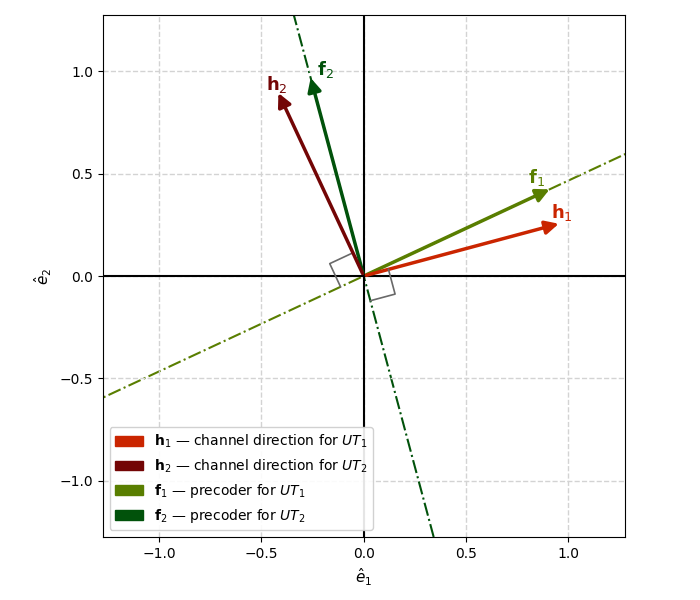
\includegraphics[width=\textwidth]{figures/background_material/04_mu_mimo_precoding/ZF_precoder_visualization/2x2_fav.png}
        \caption{favorable channel conditions}
        \label{fig:mu_mimo_zf_precoding_2x2_fav}
    \end{subfigure}
    \hfill
    \begin{subfigure}{0.495\textwidth}
        \centering
        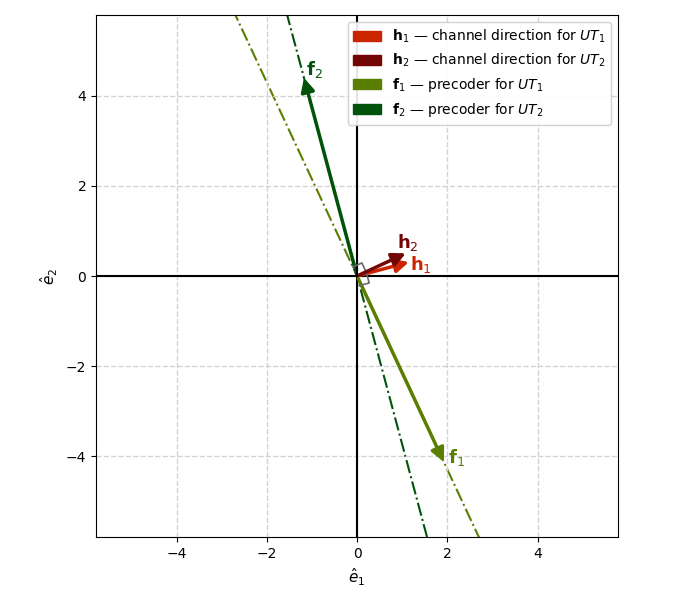
\includegraphics[width=\textwidth]{figures/background_material/04_mu_mimo_precoding/ZF_precoder_visualization/2x2_unfav.png}
        \caption{unfavorable channel conditions}
        \label{fig:mu_mimo_zf_precoding_2x2_unfav}
    \end{subfigure}
    \caption[Visualization of \ac{ZF} precoding ($2$-antenna \ac{BS} and $2$ single-antenna \acp{UT})]
    {Visualization of \ac{ZF} precoder for a \ac{MU}-\ac{MIMO} system with $2$ single-antenna \acp{UT} and a $2$-antenna \ac{BS} under (a) favorable and (b) unfavorable channel conditions.
    For both scenarios, the channel vectors are normalized and the precoding vectors are scaled such that the effective channel gain for each data stream is equal to 1.
    Note the much larger norm of the precoding vectors in the unfavorable scenario compared to the favorable scenario, which illustrates that a lot more power is required to achieve the same effective channel gain when the channel vectors of the \acp{UT} are strongly correlated.
    }
    \label{fig:mu_mimo_zf_precoding_2x2}
\end{figure}

Figure~\ref{fig:mu_mimo_zf_precoding_3x2} illustrates what happens when the \ac{BS} is equipped with an additional transmit antenna while the number of single-antenna \acp{UT} remains equal to two.
The channel matrix is still formed by two row vectors, one for each user, and the precoder by two column vectors.
However, these vectors now lie in a three-dimensional space.
As a result, the null-space orthogonal to each user's channel direction is no longer a line but a two-dimensional plane.

In order to eliminate all interference, the precoding vector for each user can be chosen anywhere in the null-space of the other users' channel vectors, that is, in the plane orthogonal to the channel directions of the other users.
The best choice is to select the precoding vectors as close as possible to the intended channel directions, which corresponds to projecting the channel vectors onto the respective orthogonal planes.
This maximizes the effective channel gain for each data stream, since it allows as much power as possible to be transmitted in the direction of the intended \ac{UT}.

\begin{figure}[!htbp]
    \centering
    \begin{subfigure}[c]{0.65\textwidth}
        \centering
        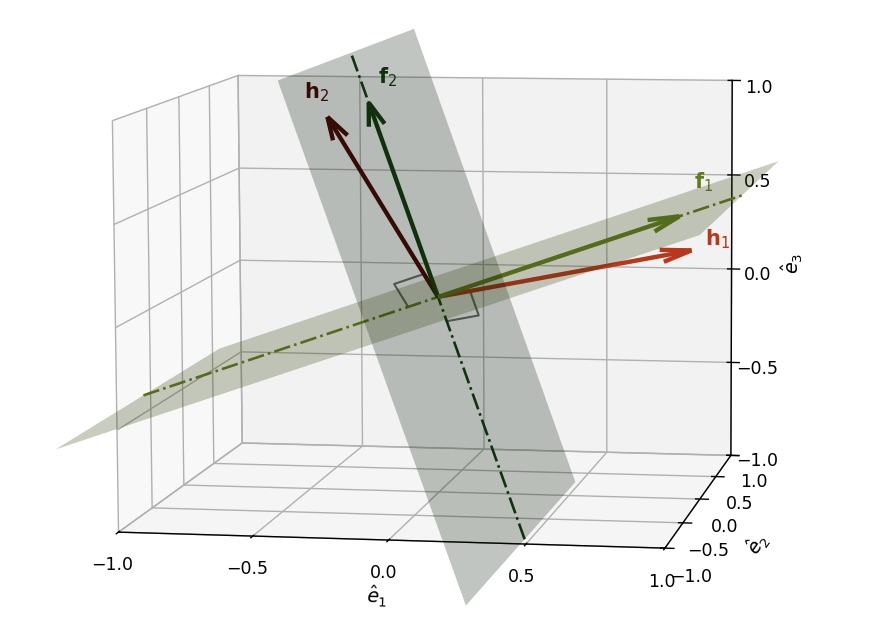
\includegraphics[width=\textwidth]{figures/background_material/04_mu_mimo_precoding/ZF_precoder_visualization/3x2_fav.jpeg}
        \label{fig:mu_mimo_zf_precoding_3x2_fav}
    \end{subfigure}
    \hfill
    \begin{subfigure}[c]{0.3\textwidth}
        \centering
        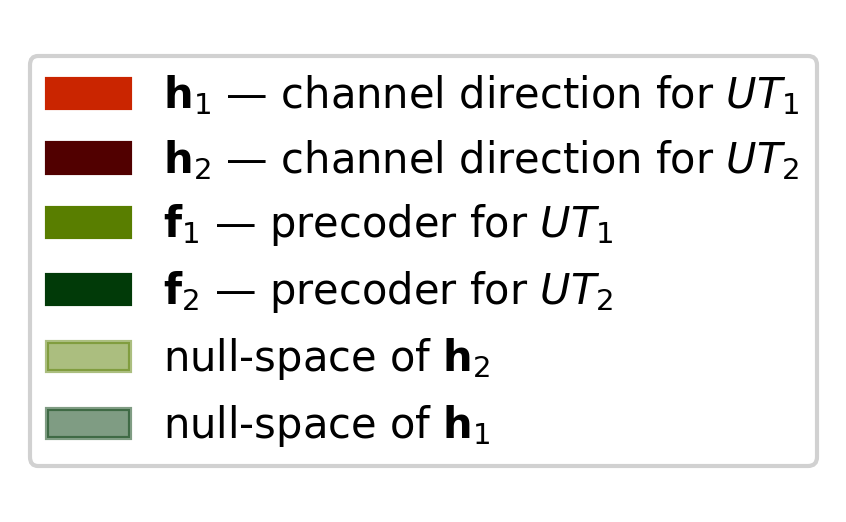
\includegraphics[width=\textwidth]{figures/background_material/04_mu_mimo_precoding/ZF_precoder_visualization/legend_3x2.png}
        \label{fig:mu_mimo_zf_precoding_legend_3x2}
    \end{subfigure}
    \caption[Visualization of \ac{ZF} precoding ($3$-antenna \ac{BS} and $2$ single-antenna \acp{UT})]
    {Visualization of \ac{ZF} precoder for a \ac{MU}-\ac{MIMO} system with $2$ single-antenna \acp{UT} and a $3$-antenna \ac{BS}.
    The channel vectors are normalized and the precoding vectors are scaled such that the effective channel gain for each data stream is equal to 1.
    With three transmit antennas, the null-space orthogonal to each user's channel direction is two-dimensional.
    The \ac{ZF} precoding vector is chosen as the projection of the intended user's channel direction onto this plane, which minimizes the deviation from the desired channel direction while preserving the zero-forcing constraint.}
    \label{fig:mu_mimo_zf_precoding_3x2}
\end{figure}

The performance of the \ac{ZF} precoding technique, in terms of the maximum sum--rate, will be discussed in the next section.

\section{Zero-Forcing Precoding with Heuristic LSV Combiner}
\label{section:mu_mimo_zf_lsv}
% =================================================
%     Zero-Forcing with Heuristic LSV Combiner
% =================================================




%% TO DO %%
% ZF+LSV precoder + In summary: algorithm for ZF+LSV precoder
% rate performance

\section{Block Diagonalization}
\label{section:mu_mimo_bd}
% =================================================
%     Block Diagonalization
% =================================================

% Coordinated vs Non-Coordinated precoding

\section{Weighted Minimum Mean Square Error}
\label{section:mu_mimo_wmmse}
% =================================================
%     Weighted Minimum Mean Square Error
% =================================================


\section{Performance Comparison}
\label{section:mu_mimo_performance_comparison}
% =============================
%     Performance Comparison
% =============================
